\documentclass[aspectratio=169,10pt]{beamer}
\usepackage{amsmath,amssymb,booktabs,graphicx,tikz}
\usetikzlibrary{arrows.meta,positioning}
\usetheme{Madrid}
\setbeamertemplate{blocks}[default]
\setbeamertemplate{title page}[default][rounded=false,shadow=false]
\definecolor{Navy}{HTML}{17365D}
\definecolor{Teal}{HTML}{168C8C}
\definecolor{Orange}{HTML}{D97706}
\setbeamercolor{structure}{fg=Navy}
\setbeamercolor{frametitle}{fg=white,bg=Navy}
\setbeamercolor{block title}{fg=Navy,bg=Navy!12}
\setbeamercolor{block body}{bg=Navy!4}
\setbeamercolor{palette primary}{fg=white,bg=Navy}
\setbeamertemplate{navigation symbols}{}
\setbeamertemplate{footline}{%
  \leavevmode\hbox{%
    \begin{beamercolorbox}[wd=.82\paperwidth,ht=2.7ex,dp=1.2ex,leftskip=1em]{palette primary}
      Problem 4: Financial SDEs\hfill 10-minute main presentation
    \end{beamercolorbox}%
    \begin{beamercolorbox}[wd=.18\paperwidth,ht=2.7ex,dp=1.2ex,center]{palette primary}
      \insertframenumber/15
    \end{beamercolorbox}}}
\newcommand{\E}{\mathbb E}
\newcommand{\dd}{\,\mathrm d}
\newcommand{\takeaway}[1]{\begin{block}{Takeaway}\small #1\end{block}}
\newcommand{\plot}[2][.67]{\centering\includegraphics[width=.93\textwidth,height=#1\textheight,keepaspectratio]{assets/#2}\par}
% Replace ONLY after the team confirms its assigned number.
\newcommand{\TeamNumber}{pending confirmation}
\newcommand{\GBMEMRate}{0.500}
\newcommand{\GBMEMWeakRate}{0.999}
\newcommand{\GBMMilRate}{0.991}
\newcommand{\GBMMilWeakRate}{1.000}
\newcommand{\GBMAnalyticWeakRate}{0.9993}
\newcommand{\GBMFitWindow}{$N=64,128,256,512,1024$}
\newcommand{\GBMExactMean}{105.1987}
\newcommand{\GBMExactVariance}{1045.0120}
\newcommand{\GBMExactMeanCI}{[105.0403, 105.3571]}
\newcommand{\NARate}{0.491}
\newcommand{\NAFitWindow}{$N=8,16,32,64$}
\newcommand{\NAExactMean}{105.08796}
\newcommand{\NAExactMeanCI}{[104.89962, 105.27629]}
\newcommand{\NAPayoff}{14.53804}
\newcommand{\NAPayoffCI}{[14.40515, 14.67093]}
\newcommand{\NAWeakInterpretation}{The 95\% intervals include zero at $N=64,128,256$. No weak order is assigned to the complete grid range. The finest-reference payoff is estimated as 14.53804 with interval [14.40515, 14.67093].}
\newcommand{\NAReferenceInterpretation}{The last refinement discrepancy is 0.04016. It is 3.2\% to 8.9\% of the coarse strong differences on the prespecified fitting window. This meets the practical 10\% reference-sensitivity criterion used for that window. For $N=256$, the ratio is 18.0\%, so the finest coarse points are retained as sensitivity evidence, not used for the principal rate claim. The two refinements decrease the strong discrepancy; their paired payoff intervals assess whether the benchmark changes at a detectable weak scale. Neither a small refinement difference nor a zero-containing interval is a rigorous bound on the unknown continuous-time error.}


\title[Financial SDEs]{Financial SDEs:\\Exact Benchmarks and Numerical References}
\subtitle{Problem 4 submission presentation}
\author{\texorpdfstring{\small
  Yifan Chen (2362353)\quad Zeya Hu (2362375)\\[.25em]
  Yanle Li (2363600)\quad Qingwen Ma (2361052)\\[.25em]
  Chenyi Xu (2359968)}{Yifan Chen, Zeya Hu, Yanle Li, Qingwen Ma, Chenyi Xu}}
\institute{Numerical Partial Differential Equations}
\date{Team number: \TeamNumber}
\pdfstringdefDisableCommands{\def\translate#1{#1}}

\begin{document}

% 1: 15 seconds.
\begin{frame}
  \titlepage
  \vspace{-1.1em}
  \centering\small Our question: how do we distinguish numerical error from sampling noise?
\end{frame}

% 2: 35 seconds.
\begin{frame}{Two models answer two different questions}
  \begin{columns}[T]
    \column{.48\textwidth}
    \begin{block}{GBM: an exact benchmark}
      \begin{itemize}
        \item A closed-form solution is available.
        \item Compare price-based EM and Milstein.
        \item Check strong and weak convergence.
      \end{itemize}
    \end{block}
    \column{.48\textwidth}
    \begin{block}{Non-affine stochastic volatility}
      \begin{itemize}
        \item No practical exact transition is available.
        \item Use EM on log price and volatility factor.
        \item Check a nested numerical reference.
      \end{itemize}
    \end{block}
  \end{columns}
  \vspace{.5em}
  \takeaway{First verify the method against an exact answer. Then test it without one.}
\end{frame}

% 3: 40 seconds.
\begin{frame}{A smaller time step solves only one part of the problem}
  \begin{columns}[T]
    \column{.48\textwidth}
    \begin{block}{Strong: compare individual paths}
      \[e_{\rm strong}(h)=\E|S_T^h-S_T|\]
      Reuse the same Brownian path in both values.
    \end{block}
    \column{.48\textwidth}
    \begin{block}{Weak: compare an expectation}
      \[e_{\rm weak}(h)=|\E\varphi(S_T^h)-\E\varphi(S_T)|\]
      State the observable $\varphi$ before reporting an order.
    \end{block}
  \end{columns}
  \[\text{sample estimate}-\text{target}
     =\text{time-step bias}+\text{Monte Carlo noise}.\]
  \takeaway{Refining $h$ reduces bias. Increasing the path count reduces sampling noise.}
\end{frame}

% 4: 40 seconds.
\begin{frame}{GBM provides an exact, coupled test}
  \[\dd S_t=\mu S_t\dd t+\sigma S_t\dd W_t,\qquad
    S_T=S_0e^{(\mu-\sigma^2/2)T+\sigma W_T}.\]
  \begin{align*}
    \text{EM:}\quad S_{n+1}&=S_n(1+\mu h+\sigma\Delta W_n),\\
    \text{Milstein:}\quad S_{n+1}&=S_n\left[1+\mu h+\sigma\Delta W_n
                  +\tfrac12\sigma^2(\Delta W_n^2-h)\right].
  \end{align*}
  \small Self-selected benchmark: $S_0=100$, $\mu=.05$, $\sigma=.30$, $T=1$.
  
  Both methods and the exact endpoint use the same increments; $\Delta W_n\sim N(0,h)$.
  \takeaway{The zero-mean Milstein correction improves pathwise accuracy, not every statistic.}
\end{frame}

% 5: 45 seconds.
\begin{frame}{GBM strong error supports the expected two orders}
  \plot{report_gbm_strong.pdf}
  \vspace{-.5em}
  \takeaway{Fitted slopes: EM $\GBMEMRate$; Milstein $\GBMMilRate$.
  Production fit: $N=64$--$1024$; $160{,}000$ paths. Independent-seed rate checks are in the Q\&A backup.}
\end{frame}

% 6: 45 seconds.
\begin{frame}{Why do both GBM weak-mean slopes equal one?}
  The observable here is the terminal price itself: $\varphi(s)=s$.
  \begin{block}{The correction has conditional mean zero}
    $\E[\Delta W_n]=0$ and $\E[\Delta W_n^2-h]=0$, so both updates satisfy
    \[\E[S_{n+1}\mid S_n]=(1+\mu h)S_n.\]
  \end{block}
  After $N=T/h$ steps, \emph{both} numerical means are $S_0(1+\mu h)^N$.
  The exact mean is $m=S_0e^{\mu T}$, and
  \[\E[S_N]-m=-\tfrac12m\mu^2Th+O(h^2).\]
  \takeaway{For our nonzero drift, both mean biases are the same and proportional to $h$.
  The curves should overlap. This equality is specific to the mean.}
\end{frame}

% 7: 35 seconds.
\begin{frame}{The weak plot confirms identical mean bias}
  \plot{report_gbm_weak.pdf}
  \vspace{-.5em}
  \takeaway{MC slopes $\GBMEMWeakRate$ and $\GBMMilWeakRate$ agree with the analytic order-one bias.
  Controls are fitted on a separate pilot; plotted estimates are not replaced by the exact bias.}
\end{frame}

% 8: 30 seconds.
\begin{frame}{Distribution and positivity provide additional checks}
  \plot[.60]{gbm_distribution.pdf}
  \vspace{-.5em}
  \small Mean and variance are also checked against the exact lognormal formulas.
  No negative terminal prices occurred on the reported grids; no clipping was used.
  \takeaway{Agreement with the distribution matters. Zero observed negatives does not prove that EM always stays positive.}
\end{frame}

% 9: 35 seconds.
\begin{frame}{Compare computational cost at the same accuracy target}
  \IfFileExists{assets/submission_cost_accuracy.pdf}{\plot[.65]{submission_cost_accuracy.pdf}}{%
    \begin{block}{Measured-cost experiment is being prepared}
      Compare EM and Milstein against the same exact GBM endpoint.
      Match terminal strong $L^1$ error before comparing cost.
    \end{block}}
  \vspace{-.4em}
  \takeaway{Both methods must meet the same error tolerance ($0.25$ currency units).
  Cost is kernel-only wall time; actual achieved errors need not be identical.}
\end{frame}

% 10: 40 seconds.
\begin{frame}{A non-affine model requires numerical integration}
  \begin{align*}
    \dd X_t&=\left(\mu-\tfrac12g(Y_t)^2\right)\dd t+g(Y_t)\dd W_t^{(1)},
      &S_t&=e^{X_t},\\
    \dd Y_t&=\kappa(\theta-Y_t)\dd t+\xi\sqrt{1+Y_t^2}\dd W_t^{(2)},
      &g(y)&=.1+\frac{.4}{1+e^{-y}}.
  \end{align*}
  \begin{itemize}
    \item $Y$ changes the volatility of the log price $X$.
    \item Both EM updates use the old value $Y_n$.
    \item Correlated increments have prescribed correlation $\rho=-.7$.
    \item Recovering $S=e^X$ preserves positivity in exact arithmetic;
      finite, positive states are also checked in the implementation.
  \end{itemize}
  \takeaway{We use the problem-pack benchmark. The scalar Milstein order-one claim is not transferred to this two-noise model.}
\end{frame}

% 11: 45 seconds.
\begin{frame}{Nested grids reuse the same noise, not the same states}
  \centering
  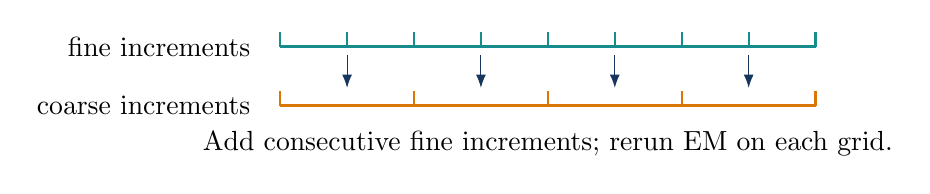
\begin{tikzpicture}[x=.85cm,y=.75cm,>=Latex]
    \foreach \i in {0,...,8}{\draw[Teal,thick] (\i,1.8)--(\i,2.05);}
    \draw[Teal,thick] (0,1.8)--(8,1.8);
    \node[anchor=east] at (-.3,1.8) {fine increments};
    \foreach \i in {0,2,4,6,8}{\draw[Orange,thick] (\i,.8)--(\i,1.05);}
    \draw[Orange,thick] (0,.8)--(8,.8);
    \node[anchor=east] at (-.3,.8) {coarse increments};
    \foreach \i in {0,2,4,6}{\draw[->,Navy] (\i+1,1.65)--(\i+1,1.1);}
    \node at (4,.15) {Add consecutive fine increments; rerun EM on each grid.};
  \end{tikzpicture}
  \vspace{.3em}
  \begin{itemize}
    \item Coarse grids: $N=8$--$256$; references: $2048$, $4096$, $8192$.
    \item $100{,}000$ paired paths. The main reference uses $8192$ steps.
    \item Strong discrepancy: $\E|S_T^N-S_T^{8192}|$.
  \end{itemize}
  \takeaway{Common noise isolates grid differences. The fine reference is still numerical, not exact.}
\end{frame}

% 12: 40 seconds.
\begin{frame}{Non-affine strong evidence is stable under refinement}
  \plot{report_nonaffine_strong.pdf}
  \vspace{-.5em}
  \takeaway{Production slopes $0.496$, $0.493$, $\NARate$ use $N=8,16,32,64$.
  Two reference refinements support half-order behaviour; they do not bound the unknown exact error.}
\end{frame}

% 13: 40 seconds.
\begin{frame}{The nonlinear payoff reveals a weak-resolution limit}
  \plot[.58]{report_nonaffine_weak.pdf}
  \vspace{-.5em}
  \small Paired payoff: $\varphi(s)=(s-100)^+$; undiscounted, not a risk-neutral option price.
  \takeaway{Fine-grid confidence intervals include zero. We do not claim a reliable weak order.
  The log-EM mean is exact in expectation, so it cannot test weak convergence here.}
\end{frame}

% 14: 30 seconds.
\begin{frame}{Diagnostics and reproducibility support the plots}
  \begin{tabular}{p{.31\textwidth}p{.60\textwidth}}
    \toprule
    Check & Evidence \\
    \midrule
    Brownian inputs & Increment variances match $h$; correlation $-.699675$ matches target $-.7$.\\
    Model states & Finite-state and positivity checks pass on reported grids.\\
    Structural oracle & Non-affine theoretical mean is inside the sampled mean interval.\\
    Reference sensitivity & Three numerical references; two successive refinement tests.\\
    Reproduction & Fixed seeds, recorded environments, one run script, saved tables and checks.\\
    \bottomrule
  \end{tabular}
  \takeaway{A clear convergence line is useful only when the inputs, reference, and uncertainty are checked.}
\end{frame}

% 15: 35 seconds. Main presentation ends here (550 seconds of speech nominal).
\begin{frame}{Main conclusions: accuracy depends on what we measure}
  \begin{enumerate}
    \item In GBM, Milstein improves strong order from one-half to one.
    \item The two methods have identical first-order weak bias for the mean.
    \item Nested-grid log-EM gives stable half-order strong evidence for the non-affine model.
    \item The nonlinear weak-payoff rate remains unresolved at the current sampling budget.
  \end{enumerate}
  \vspace{.7em}
  \takeaway{Use exact benchmarks where possible. Otherwise refine the reference, couple the paths, and report the limits of the evidence.}
  \centering\small Thank you. Questions?
\end{frame}

\appendix
\setbeamertemplate{footline}{%
  \begin{beamercolorbox}[wd=\paperwidth,ht=2.7ex,dp=1.2ex,leftskip=1em]{palette primary}
    Problem 4: Financial SDEs\hfill Q\&A backup -- outside the timed main talk\hspace{1em}
  \end{beamercolorbox}}
\begin{frame}[noframenumbering]{Q\&A backup: sources and reproducibility}
  \begin{thebibliography}{9}
    \bibitem{pack}Course Problem Pack, Problem 4: Financial SDEs, pp.~6--7.
    \bibitem{higham}D. J. Higham, \emph{An Algorithmic Introduction to Numerical Simulation
      of Stochastic Differential Equations}, SIAM Review 43(3), 2001, pp.~525--546.
    \bibitem{kp}P. E. Kloeden and E. Platen, \emph{Numerical Solution of Stochastic
      Differential Equations}, Springer, 1992.
  \end{thebibliography}
  \small Submission code: \texttt{code/run\_all.py}, \texttt{code/verify.py}, and the supplied README.
  
  This slide is for the three-minute Q\&A and is not part of the timed main presentation.
  \takeaway{Every numerical conclusion should be traceable to a reproducible experiment.}
\end{frame}

\begin{frame}[noframenumbering]{Q\&A backup: why the non-affine mean is not a weak test}
  Conditional on the old state, $g_n=g(Y_n)$ is known. Log-EM gives
  \[S_{n+1}=S_n\exp\!\left[(\mu-\tfrac12g_n^2)h+g_n\Delta W_{1,n}\right].\]
  For a Gaussian increment, $\E[e^{g_n\Delta W_{1,n}}\mid\mathcal F_n]=e^{g_n^2h/2}$, so
  \[\E[S_{n+1}\mid\mathcal F_n]=S_ne^{\mu h},\qquad
    \E[S_N]=S_0e^{\mu T}.\]
  Correlation between the two drivers does not change this conditional calculation.
  \takeaway{An exact mean does not imply an exact terminal distribution. A nonlinear payoff probes a different statistic.}
\end{frame}

\begin{frame}[noframenumbering]{Q\&A backup: GBM slopes repeated with independent seeds}
  \plot[.67]{submission_gbm_repeat_slopes.pdf}
  \vspace{-.5em}
  \takeaway{Eight independent seeds, $5{,}000$ production paths per seed and an independent pilot.
  Shading shows empirical cross-seed curve spread, not a guaranteed population confidence band.}
\end{frame}

\begin{frame}[noframenumbering]{Q\&A backup: the non-affine slope is also repeatable}
  \plot[.67]{submission_nonaffine_repeat_slopes.pdf}
  \vspace{-.5em}
  \takeaway{Eight independent seeds, $1{,}000$ paths each, and the same $8192$-step reference protocol.
  The fitted slope averages $0.498$ (cross-seed SD $0.017$); this is a smaller-budget repeat check.}
\end{frame}

\end{document}
